\nocite{*} %wszystkie wpisy trafią do bibliografii
\lstset{language=Java, tabsize=2,  basicstyle=\footnotesize\ttfamily, keywordstyle=\underbar}

% \setpagenumberingtype{gobble} % Remove page numbers (and reset to 1)
\setcounter{page}{1}
\newgeometry{tmargin=3cm, bmargin=3cm, lmargin=2cm, rmargin=2cm}

% \newgeometry{tmargin=3cm, bmargin=3cm, lmargin=2cm, rmargin=2cm}

\thispagestyle {empty}

\begin{center}
	%logo uczelni
	
\includegraphics[scale=0.4]{img/pw}
	
	\vspace{0.5cm}
	
	{\fontsize{20}{20}\selectfont POLITECHNIKA WARSZAWSKA}
	
	\vspace{1.0cm}
	
	\textbf{{\fontsize{14}{14}\selectfont Wydział Mechatroniki}}
	
	\vspace{1.5cm}
	
	\textbf{{\fontsize{14}{14}\selectfont Praca magisterska}}

	\vspace{2.0cm}
	
	{\fontsize{14}{14}\selectfont Ireneusz Szulc}
	
	\vspace{1cm}
	
	{\fontsize{28}{28}\selectfont Planowanie bezkolizyjnych tras dla zespołu robotów mobilnych}
	
	\vspace{1cm}
	\begin{flushright}
		{\fontsize{14}{14}\selectfont Opiekun pracy: \\ 
		prof. nzw. dr hab. Barbara Siemiątkowska
		}
	
		\vspace{1cm}
		
		\vspace{3cm}
		% {\fontsize{14}{14}\selectfont Konsultant pracy: \\ 
		% mgr inż. }
		
	\end{flushright}
	
	\vspace{1cm}
	
	{\fontsize{12}{12}\selectfont Warszawa, 2018}
	
	%\cleardoublepage %nie działa
	
	%\clearpage\mbox{}\clearpage
\end{center}
% \clearpage{\pagestyle{empty}\cleardoublepage}
% \clearpage

% \phantomsection
% \addcontentsline{toc}{chapter}{Spis treści}
% \tableofcontents
% \clearpage

\raggedbottom
% \setpagenumberingtype{arabic} % kontynuowanie numerowania w stylu arabskim

\chapter{Karta tematu}
\label{ch:topic}

Karta tematu: \\
Temat pracy: Planowanie bezkolizyjnych tras dla zespołu robotów mobilnych \\
Temat pracy (w jęz. ang.): Path planning for a group of mobile robots

Zakres pracy:
\begin{itemize}
	\item Projekt algorytmu wyznaczania trajektorii dla pojedynczego robota
	\item Algorytm detekcji i zapobiegania kolizjom między robotami
	\item Implementacja oprogramowania symulacyjnego
	\item Przeprowadzenie testów symulacyjnych
\end{itemize}

Podstawowe wymagania:
\begin{itemize}
	\item Aplikacja powinna umożliwiać symulację ruchu robotów oraz definiowanie położenia przeszkód przez użytkownika.
	\item Planowanie tras dotyczy robotów holonomicznych.
\end{itemize}

Założenia:
• The environment is deterministic. However, agents may not move if they are trying to move to an obstacle or another agent.
• For simplicity, agents only have the path finding task. Moreover, the agents won’t disappear when they reach their target. They just stay at the target block and the block cannot be used by other agents.
• No two agents can have the same target.
• Agents have a full view of the map and other agents.
• Actions are: lewo, prawo, góra, dół i na ukosy w labiryncie

\chapter{Konspekt pracy}
\label{ch:konspekt}
\begin{itemize}
	\item Wstęp teoretyczny:
	\begin{itemize}
		\item Cooperative Pathfinding
		\item algorytm A* - szczegółowo
		\item przegląd metod planowania tras dla wielu robotów
		\item artykuł o Cooperative Pathfinding, time-space A*
		\item artykuł o wyznaczaniu priorytetów i metodach planowania tras (prezentacja): Path Coordination, time-space A*
		\item metoda ładunków - problem minimów lokalnych
		\item replanowanie po wykruciu kolizcji (algorytm D*)
		\item algorytmy WHCA* i IADPP
		\item Reciprocal Collision Avoidance
		\item metody przydziału priorytetów - zwiększanie i przeliczanie
		\item metody zcentralizowane vs rozproszone (porównanie)
		\item time-space A*, heurystyki, Reservation Table
	\end{itemize}
	\item zastosowanie: ciasne korytarze, częsty problem kolizji, szpitale, transport dokumentów, paczek
	\item generowanie mapy - labiryntu do testów: własny algorytm, teoria grafów, własności mapy
	\item time-space A* - pseudokod, schemat blokowy, własne heurystyki, modyfikacje
	\item metoda przydziału / zmiany priorytetów
	\item ograniczenia - nałożone uproszczenia: ruch skośny, czas dyskretny, brak czasu na obrót
	\item Implementacja aplikacji - stack technologiczny: Java 8, Java FX, Spring, Spring Boot, testy jednostkowe jUnit, git, IntelliJ, Maven, Linux; schemat klas aplikacji
	\item obszerne testy, porównanie wyników metod przy tych samych warunkacj początkowych
\end{itemize}
\clearpage{\pagestyle{empty}\cleardoublepage}

% \chapter{Wstęp}
\label{ch:wstep}

\section{Cel i zakres pracy}
Przedmiotem niniejszej pracy jest przegląd metod wykorzystywanych do planowania bezkolizyjnych tras dla wielu robotów mobilnych.
Stanowi to również wstęp teoretyczny do zaprojektowania algorytmu i implementacji oprogramowania pozwalającego na symulację działania skutecznego planowania tras dla systemu wielorobotowego.

Praca skupia się na przypadkach, w których mamy do czynienia ze środowiskiem z dużą liczbą przeszkód (np. zamknięty budynek z licznymi ciasnymi korytarzami), aby uwypuklić  problem blokowania sią agentów często prowadzący do zakleszczenia. Często okazuje się, że należy wtedy zastosować nieco inne podejścia niż te, które sprawdzają się w przypadku otwartych środowisk, a które zostały opisane np. w pracach \cite{roszkowska}, \cite{siemiatkowska}.
W otwartych środowiskach z małą liczbą przeszkód wystarczające może się okazać np. proste replanowanie wykorzystujące algorytm D* (por. \ref{ch:dstar}) lub LRA* (por. \ref{ch:lra}).

W niniejszej pracy starano się znaleźć metody rozwiązujące zagadnienie, w którym znane są:
\vspace{-1em}
\begin{itemize}[noitemsep]
	\item pełna informacja o mapie otoczenia (położenie statycznych przeszkód),
	\item aktualne położenie i położenie celu każdego z robotów.
\end{itemize}
Szukany jest natomiast przebieg tras do punktów docelowych dla agentów. Zadaniem algorytmu będzie wyznaczenie możliwie najkrótszej bezkolizyjnej trasy dla wszystkich robotów. Należy jednak zaznaczyć, że priorytetem jest dotarcie każdego z robotów do celu bez kolizji z innymi robotami. Drugorzędne zaś jest, aby wyznaczone drogi były możliwie jak najkrótsze.

\clearpage
\subsection{Założenia}
\label{ch:zalozenia}
Założenia i ograniczenia rozważanego problemu:
\begin{enumerate}
	\item Każdy z robotów ma wyznaczony inny punkt docelowy, do którego zmierza.
	\item Planowanie tras dotyczy mobilnych robotów holonomicznych.
	\item Czas trwania zmiany kierunku robota jest pomijalnie mały.
	\item Srodowisko, w którym poruszają się roboty, jest dwuwymiarową przestrzenią zawierającą dużą liczbę przeszkód oraz wąskie korytarze (por. rys. \ref{fig:img_robopath_sample-maze}).
	\item Roboty "wiedzą" o sobie i mogą komunikować się ze sobą podczas planowania tras.
	\item Każdy robot zajmuje w przestrzeni jedno pole. Na jednym polu może znajdować się maksymalnie jeden robot (por. rys. \ref{fig:img_robopath_sample-maze}).
	\item Planowanie tras powinno odbywać się w czasie rzeczywistym.
\end{enumerate}

\begin{figure}[H]
	\centering
	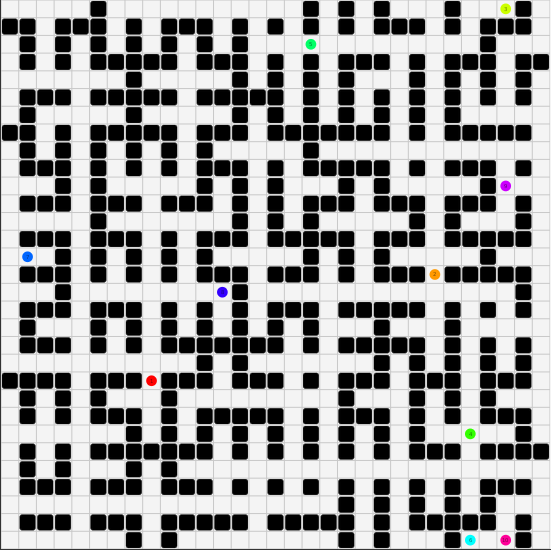
\includegraphics[width=8cm]{img/robopath/sample-maze}
	\caption{Przykładowe środowisko z dużą liczbą przeszkód i rozmieszczonymi robotami. Źródło: własna implementacja oprogramowania symulacyjnego}
	\label{fig:img_robopath_sample-maze}
\end{figure}


\clearpage
\section{Koordynacja ruchu robotów}
Koordynacja ruchu robotów jest jednym z fundamentalnych problemów w systemach wielorobotowych. \cite{optpriorities}

Kooperacyjne znajdowanie tras (ang. {\it Cooperative Pathfinding}) jest zagadnieniem planowania w układzie wieloagentowym, w którym to agenci mają za zadanie znaleźć bezkolizyjne drogi do swoich, osobnych celów. Planowanie to odbywa się w oparciu o pełną informację o środowisku oraz o trasach pozostałych agentów. \cite{cooppath}

Algorytmy do wyznaczania bezkolizyjnych tras dla wielu agentów (robotów) mogą znaleźć zastosowanie w szpitalach (np. roboty TUG i HOMER do dostarczania sprzętu na wyposażeniu szpitala \cite{tughomer}) oraz magazynach (np. roboty transportowe w magazynach firmy Amazon \ref{fig:image_kiva_amazon}).

\begin{figure}[H]
	\centering
	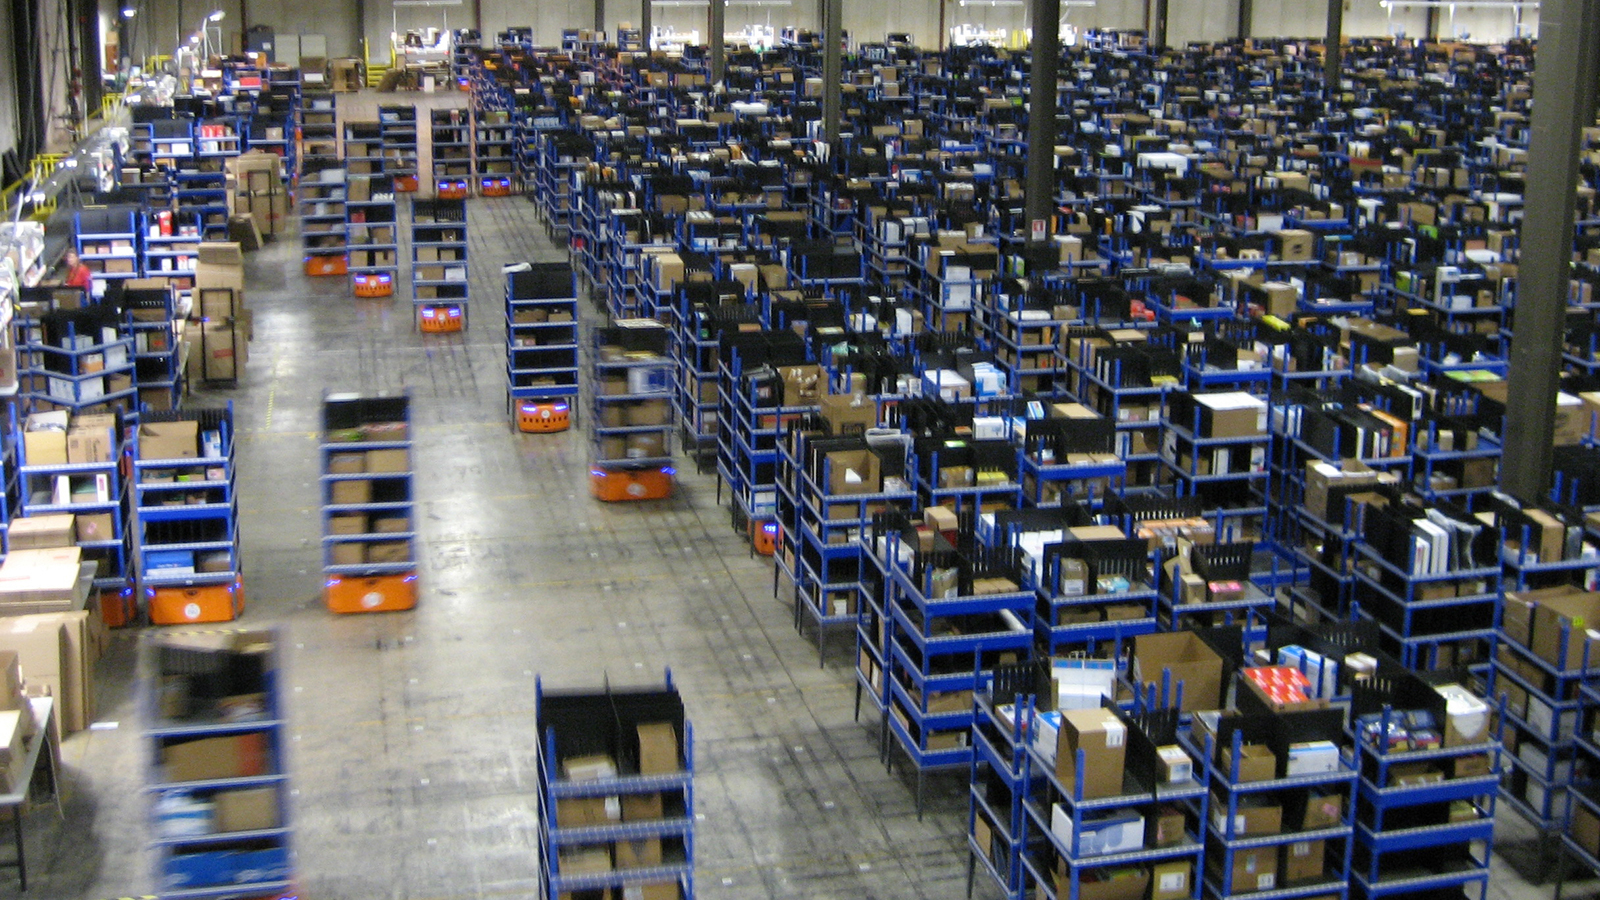
\includegraphics[width=14cm]{img/kiva-amazon}
	\caption{Roboty Kiva pracujące w magazynie firmy Amazon. Źródło: \cite{amazonkiva}}
	\label{fig:image_kiva_amazon}
\end{figure}

\subsection{Podobieństwo do gier RTS}
Problem kooperacyjnego znajdowania tras pojawia się nie tylko w robotyce, ale jest również popularny m.in. w grach komputerowych (strategiach czasu rzeczywistego), gdzie konieczne jest wyznaczanie bezkolizyjnych dróg dla wielu jednostek, unikając wzajemnego blokowania się. Niestety brak wydajnych i skutecznych algorytmów planowania dróg można zauważyć w wielu grach typu RTS (ang. {\it Real-Time Strategy}), gdzie czasami obserwuje się zjawisko zakleszczenia jednostek w wąskich gardłach (np. Age of Empires II, Warcraft III lub nawet we współczesnych produkcjach) \cite{efficient_coop_pathplanning} (por. rys. \ref{fig:img_games_age-deadlock}). Ponadto, zauważalny brak ogólnie dostępnych bibliotek open-source do rozwiązania problemu typu {\it Cooperative Pathfinding} świadczy o potrzebie rozwoju tych metod.

Często algorytmy wykorzystywane w grach typu RTS (ang. {\it Real-Time Strategy}) zajmują się planowaniem bezkolizyjnych dróg dla układu wielu agentów w czasie rzeczywistym (będącego przedmiotem niniejszej pracy), dlatego nic nie stoi na przeszkodzie, aby stosować je zamiennie również do koordynacji ruchu zespołu robotów mobilnych.

\begin{figure}[H]
	\centering
	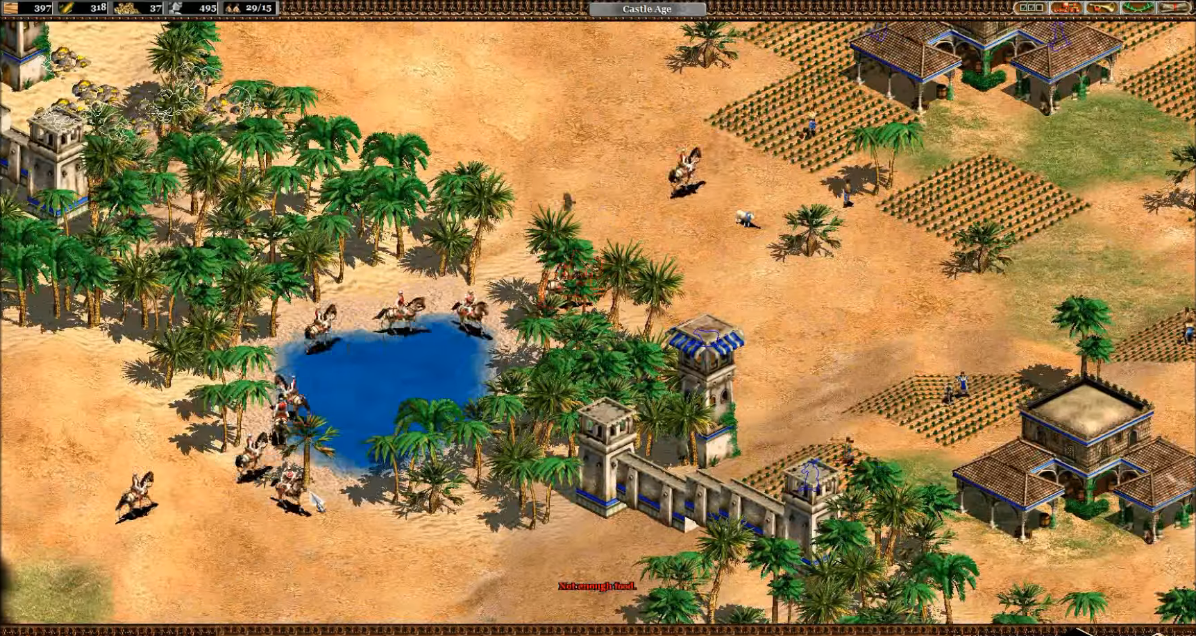
\includegraphics[width=14cm]{img/games/age-deadlock}
	\caption{Popularny problem zakleszczania się jednostek w wąskich gardłach występujący w grach typu RTS. Źródło: gra komputerowa Age of Empires II HD}
	\label{fig:img_games_age-deadlock}
\end{figure}

\section{Podstawowe pojęcia}
\subsubsection{Robot holonomiczny}
Robot holonomiczny to taki robot mobilny, który może zmienić swoją orientację, stojąc w miejscu.

\subsubsection{Przestrzeń konfiguracyjna}
Przestrzeń konfiguracyjna to $N$-wymiarowa przestrzeń będąca zbiorem możliwych stanów danego układu fizycznego.
Wymiar przestrzeni zależy od rodzaju i liczby wyróżnionych parametrów stanu.
W odróżnieniu od przestrzeni roboczej, gdzie robot ma postać bryły, w przestrzeni konfiguracyjnej robot jest reprezentowany jako punkt.

\subsubsection{Zupełność algorytmu (ang. {\it Completeness})}
W kontekście algorytmu przeszukiwania grafu algorytm zupełny to taki, który gwarantuje znalezienie rozwiązania, jeśli takie istnieje.
Warto zaznaczyć, że nie gwarantuje to wcale, że znalezione rozwiązanie będzie rozwiązaniem optymalnym.

% TODO-MGR
% \subsubsection{Metoda hill-climbing}
% Metoda hill-climbing jest rodzajem matematycznej optymalizacji, lokalną metodą przeszukiwania.
% Jest to iteracyjny algorytm, który zaczyna w wybranym rozwiązaniu problemu, następnie próbuje znaleźć lepsze rozwiązanie poprzez przyrostowe zmiany pojedynczych elementów rozwiązania.
% Jeśli przyrostowa zmiana przynosi lepsze rozwiązanie, jest ona wprowadzana do nowego rozwiązania.
% Kroki algorytmu powtarzane są dotąd, aż żadna zmiana nie przynosi już poprawy.

% \clearpage{\pagestyle{empty}\cleardoublepage}

% \section{Kooperacyjne planowanie tras}
\label{ch:cooperative_pathfinding}

% \section{Metody planowania tras}
Spośród metod wykorzystywanych do kooperacyjnego planowania tras dla wielu robotów można wyróżnić dwie zasadnicze grupy \cite{latombe}:
\begin{itemize}
	\item {\bf Zcentralizowane} - drogi wyznaczane są dla wszystkich agentów na raz (jednocześnie). Metody tego typu są często trudne do zrealizowania (gdyż do rozwiązania jest złożony problem optymalizacyjny) oraz mają bardzo dużą złożoność obliczeniową ze względu na ogromną przestrzeń przeszukiwania. Struktura organizacyjna jest scentralizowana - decyzje podejmowane są na podstawie centralnego systemu.
	\item {\bf Rozproszone} (ang. {\it decoupled} lub {\it distributed}) - podejście to dekomponuje zadanie na niezależne lub zależne w niewielkim stopniu problemy dla każdego agenta. Dla każdego robota droga wyznaczana jest osobno, w określonej kolejności, następnie rozwiązywane są konflikty (kolizje dróg).
	Zastosowanie metod rozproszonych wiąże się najczęściej z koniecznością przydzielania priorytetów robotom, co stanowi istotny problem, gdyż od ich wyboru może zależeć zupełność algorytmu. Nie należy mylić tej metody z zagadnieniem typu {\it Non-Cooperative Pathfinding}, w którym agenci nie mają wiedzy na temat pozostałych planów i muszą przewidywać przyszłe ruchy pozostałych robotów \cite{cooppath}. W podejściu rozproszonym agenci mają pełną informację na temat stanu pozostałych robotów, lecz wyznaczanie dróg odbywa się w określonej kolejności.
\end{itemize}

W systemach czasu rzeczywistego istotne jest, aby rozwiązanie problemu planowania tras uzyskać w krótkim, deterministycznym czasie, dlatego w tego typu systemach chętniej używane są techniki rozproszone.

\section{Metoda pól potencjałowych}
\label{ch:theory-potential-fields}
Metoda pól potencjałowych (ang. {\it Artificial Potential Field} lub {\it Potential Field Technique}) polega na odwzorowaniu w ruchu robotów zasad oddziaływania między ładunkami elektrycznymi. Roboty i przeszkody reprezentowane są jako ładunki jednoimienne, przez co "odpychają się" siłą odwrotnie proporcjonalną do kwadratu odległości (dzięki temu unikają kolizji między sobą). Natomiast punkt docelowy robota jest odwzorowany jako ładunek o przeciwnym biegunie, przez co robot jest "przyciągany" do celu.
Główną zasadę działania metody przedstawiono na rysunku \ref{fig:image_potentialfield}.

Technika ta jest bardzo prosta i nie wymaga wykonywania złożonych obliczeń (w odróżnieniu do pozostałych metod zcentralizowanych).
Niestety bardzo powszechny jest problem osiągania minimum lokalnego, w którym suma wektorów daje zerową siłę wypadkową. Robot zostaje "uwięziony" w takim minimum lokalnym, przez co nie jest w stanie dotrzeć do wyznaczonego celu. Do omijania tego problemu muszą być stosowane inne dodatkowe metody \cite{potentialfield}.
Metoda pól potencjałowych nie daje gwarancji ani optymalności, ani nawet zupełności.
\begin{figure}
	\centering
	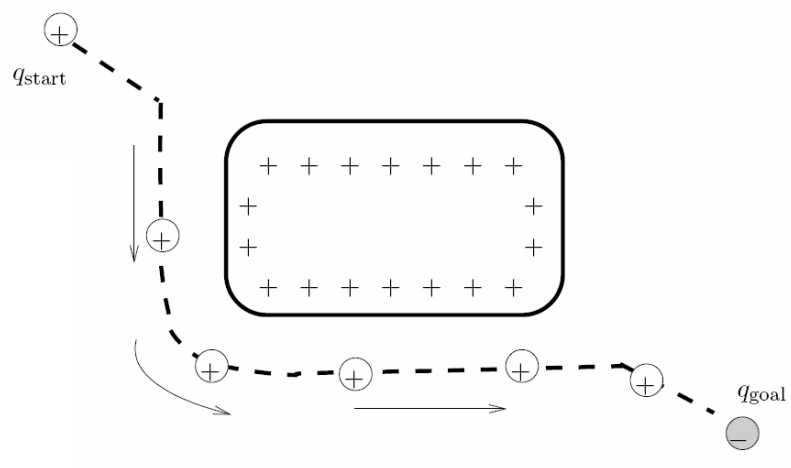
\includegraphics[width=12cm]{img/potential-field}
	\caption{Zasada działania metody pól potencjałowych. Dodatni ładunek $q_{start}$ reprezentuje robota. Przyciągany jest w stronę ujemnego ładunku celu $q_{goal}$, zaś odpychany jest od dodatnio naładowanej przeszkody. Źródło: \cite{howie_potentialfield}}
	\label{fig:image_potentialfield}
\end{figure}

\section{Rozproszone planowanie tras}
Najczęściej stosowanymi podejściami są metody oparte o algorytm A* lub jego pochodne.
W celu wykonywania wydajnych obliczeń w algorytmach przeszukujących grafy, nawet w przypadku ciągłej przestrzeni mapy, stosuje się podział na dyskretną siatkę pól (por. rys. \ref{fig:img_games_warcraft-map-editor}) \cite{hierpathfindinginrts}.

\begin{figure}[H]
	\centering
	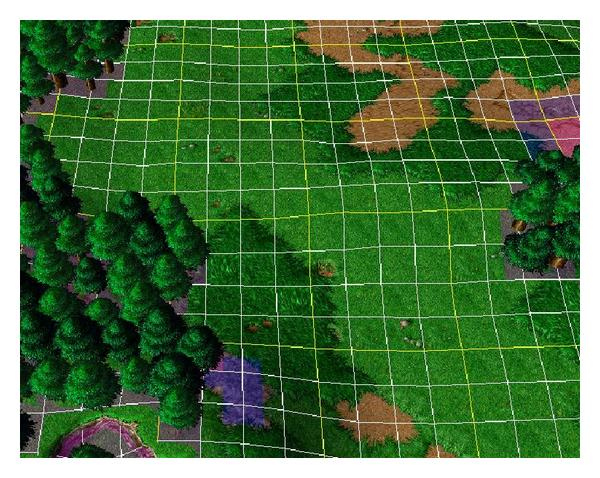
\includegraphics[width=0.5\columnwidth]{img/games/warcraft-map-editor}
	\caption{Ciągła przestrzeń mapy zdyskretyzowana do siatki pól. \\ Źródło: edytor map z gry Warcraft III.}
	\label{fig:img_games_warcraft-map-editor}
\end{figure}

Popularne podejścia unikające planowania w wysoko wymiarowej zbiorowej przestrzeni konfiguracyjnej to techniki rozproszone i uwzględniające priorytety \cite{optpriorities}.
Pomimo, że metody te są bardzo efektywne, mają dwie główne wady:
\vspace{-0.5em}
\begin{itemize}[itemsep=0em]
	\item Nie są zupełne - nie dają gwarancji znalezienia rozwiązania, nawet gdy takie istnieje.
	\item Wynikowe rozwiązania mogą być nieoptymalne.
\end{itemize}

% TODO-MGR
% W artykule \cite{optpriorities} przedstawione zostało podejście do optymalizowania układu priorytetów dla rozproszonych i uwzględniających priorytety technik planowania.
% Proponowana metoda wykonuje randomizowane przeszukiwanie z techniką hill-climbing do znalezienia rozwiązania i do skrócenia całkowitej długości ścieżek.
% Technika ta została zaimplemenotwana i przetestowana na prawdziwych robotach oraz w rozległych testach symulacyjnych, dając zadowalające rezultaty.

\section{Planowanie uwzględniające priorytety}
Często używaną w praktyce metodą jest planowanie z uwzględnianiem priorytetów. 
W tej technice agenci otrzymują unikalne priorytety. Algorytm wykonuje indywidualne planowanie sekwencyjnie dla każdego agenta w kolejności od najwyższego priorytetu. Trajektorie agentów o wyższych priorytetach są ograniczeniami (ruchomymi przeszkodami) dla pozostałych agentów \cite{async_decentralized_spacetime_cp}.

Złożoność ogólnego algorytmu rośnie liniowo wraz z liczbą agentów, dzięki temu to podejście ma zastosowanie w problemach z dużą liczbą agentów.
Algorytm ten jest zachłanny i niezupełny w takim znaczeniu, że agentów zadowala pierwsza znaleziona trajektoria niekolidująca z agentami wyższych priorytetów. 

Istotną rolę doboru priorytetów robotów w procesie planowania tras ukazuje prosty przykład przedstawiony na rysunku \ref{fig:image_article1_fig1}. Jeśli robot 1 (zmierzający z punktu S1 do G1) otrzyma wyższy priorytet niż robot 2 (zmierzający z S2 do G2), spowoduje to zablokowanie przejazdu dla robota 2 i w efekcie prawidłowe, istniejące rozwiązanie nie zostanie znalezione.
\begin{figure}
	\centering
	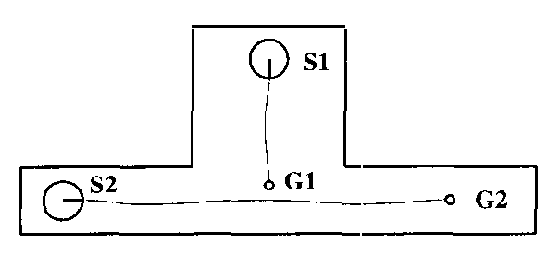
\includegraphics[width=6cm]{img/article1/fig1}
	\caption{Sytuacja, w której żadne rozwiązanie nie zostanie znalezione, stosując planowanie uwzględniające priorytety, jeśli robot 1 ma wyższy priorytet niż robot 2. Źródło: \cite{optpriorities}}
	\label{fig:image_article1_fig1}
\end{figure}

Układ priorytetów może mieć także wpływ na długość uzyskanych tras. Potwierdzający to przykład został przedstawiony na rysunku \ref{fig:image_article1_ppt6}. W zależności od wyboru priorytetów, wpływających na kolejność planowania tras, otrzymujemy różne rozwiązania.
\begin{figure}
	\centering
	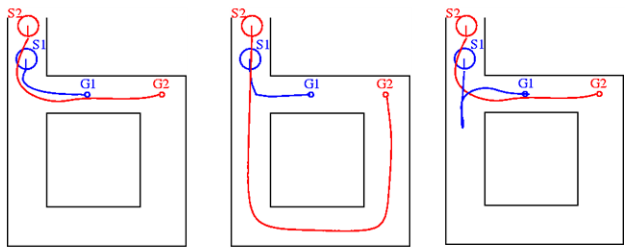
\includegraphics[width=13cm]{img/article1/ppt6}
	\caption{a) Niezależne planowanie optymalnych tras dla 2 robotów; b) suboptymalne rozwiązanie, gdy robot 1 ma wyższy priorytet; c) rozwiązanie, gdy robot 2 ma wyższy priorytet. Źródło: \cite{optpriorities}}
	\label{fig:image_article1_ppt6}
\end{figure}

\section{Metoda Path Coordination}
Jedną z metod rozproszonego planowania tras z uwzględnianiem priorytetów jest {\it Path Coordination}, której idea przedstawia się w następujących krokach \cite{optpriorities}:
\begin{enumerate}
	\item Wyznaczenie ścieżki dla każdego robota {\bf niezależnie} (np. za pomocą algorytmu A*)
	\item Przydział priorytetów
	\item Próba rozwiązania możliwych konfliktów między ścieżkami. Roboty utrzymywane są na ich indywidualnych ścieżkach (wyznaczonych na początku), wprowadzane modyfikacje pozwalają na zatrzymanie się, ruch naprzód, a nawet cofanie się, ale tylko {\bf wzdłuż trajektorii} w celu uniknięcia kolizji z robotem o wyższym priorytecie.
\end{enumerate}
% \clearpage{\pagestyle{empty}\cleardoublepage}

% \section{Wyznaczanie trajektorii dla pojedynczego robota}
\label{ch:alg-single-astar}

Wiele technik planowania tras, mimo iż może posłużyć do koordynacji ruchu wielu robotów, korzysta z metod indywidualnego planowania dla każdego agenta z osobna. Przykładem takiego podejścia jest {\it Local-Repair A*}, w którym to głównym algorytmem przeszukującym jest A*.
Z tego powodu przed przystąpieniem do opracowania bardziej skomplikowanych metod, należy najpierw zająć się implementacją algorytmu poszukiwania najkrótszej drogi na dwuwymiarowej mapie z jednym robotem. Wymagane jest to nawet dla metody WHCA*, która pomimo, że operuje na węzłąch określonych w czasie i przestrzeni, to jednak w obliczaniu samej heurystyki wykorzystuje przestrzenny algorytm A*.
Ogólna zasada działania algorytmu A* wraz z kluczowymi pojęciami została opisana w rozdziale \ref{ch:astar-theory}.

Pseudoko \ref{alg:astar} oraz opisy użytych pomocniczych funkcji ukazują szczegóły implementacji metody wyznaczania najkrótszej drogi na przestrzennej mapie. Algorytm oparty jest o A*, jednak posiada własne, niewielkie modyfikacje.

\begin{algorithm}[H]
	\caption{Algorytm A*}\label{alg:astar}
  \begin{algorithmic}[1]
\Function{znajdzDrogę}{$mapa$, $start$, $cel$}
	\State $closed \gets \varnothing$  \Comment{pusta lista zamkniętych}
	\State $open \gets \{start\}$ \Comment{lista otwartych zawiera punkt startowy}

	\For{$wezel \in mapa$}
		\State $wezel.g = \infty$ \Comment{domyślnie nieskończony koszt - odległość od startu}
	\EndFor

	\State $start.g \gets 0$ \Comment{Zerowy koszt przejścia do węzła startowego}

	\While{$open \ne \varnothing$} \Comment{dopóki lista otwartych nie jest pusta}
		\State $obecny \gets $ \Call{znajdźMinF}{$open$} \Comment{Szukamy pola o najniższej wartości f}

		\If{$obecny == cel$}
			\State \Return \Call{zbudujŚcieżkę}{$cel$} \Comment{Znaleziono ścieżkę}
		\EndIf

		\State dodaj $obecny$ do $closed$ \Comment{Przesunięcie z $open$ do $closed$}
		\State usuń $obecny$ z $open$
		
		\For{$sasiad \in$ \Call{sąsiedzi}{$obecny$}} \Comment{Dla każdego sąsiada aktualnego pola}
			
			\If{$mapa[sasiad.x][sasiad.y] == ZABLOKOWANE$ {\bf or} 
				\State {\bf not} \Call{przejściePoprawne}{$obecny$, $sasiad$}}
				\State {\bf continue} \Comment{Ignoruj niepoprawne pola lub przejścia}
			\EndIf
			
			\State $nowyKoszt \gets obecny.g \ +$ \Call{kosztPrzejścia}{$obecny$, $sasiad$}

			\If{$nowyKoszt < sasiad.g$} \Comment{znaleziono korzystniejsze połączenie}
				\State usuń $sasiad$ z $open$ \Comment{konieczność ponownego przeliczenia}
				\State usuń $sasiad$ z $closed$ \Comment{jeśli $sasiad \in open$ lub $sasiad \in closed$}
			\EndIf

			\If{$sasiad \not\in open \land sasiad \not\in closed$}
				\State $sasiad.g \gets nowyKoszt$ \Comment{zapisanie nowego połączenia}
				\State $sasiad.h \gets$ \Call{heurystyka}{$sasiad$, $cel$}
				\State $sasiad.parent \gets obecny$ \Comment{pole $obecny$ rodzicem dla pola $sasiad$}
				\State dodaj $sasiad$ do $open$
			\EndIf

		\EndFor
	\EndWhile

	\State \Return $\varnothing$ \Comment{Przeanalizowano wszystkie węzły, brak istniejącej ścieżki}
\EndFunction
  \end{algorithmic}
\end{algorithm}

Wykorzystane zostały pomocnicze funkcje:
\begin{itemize}
	\item \textsc{znajdźMinF}($lista$) - Funkcja zwraca z listy pole o najniższej wartości $f$ (sumie kosztu i heurystyki);
	\item \textsc{zbudujŚcieżkę}($cel$) - Funkcja zwraca ścieżkę z punktu startowego do punktu $cel$ zbudowaną na podstawie przechodzenia wstecz od punktu $cel$ po kolejnych rodzicach węzłów, aż do dotarcia do węzła bez rodzica (punktu startowego).
	\item \textsc{sąsiedzi}($pole$) - Funkcja zwraca zbiór pól bezpośrednio sąsiadujących (dla których istnieje możliwość przejścia) ze wskazanym polem. Jest to zazwyczaj zbiór ośmiu sąsiadujących pól. Funkcja uwzględnia warunki brzegowe na granicach mapy.
	\item \textsc{przejściePoprawne}($poleZ$, $poleDo$) - Funkcja zwraca prawdę wtedy i tylko wtedy, gdy istnieje możliwość przejścia z $poleZ$ do $poleDo$. Gdy wykonywany jest ruch ukośny, ale na przynajmniej jednym polu sąsiadującym z $poleZ$ i $poleDo$ znajduje się przeszkoda, to taki ruch jest niepoprawny. Ruch ukośny agenta z punktu $(x_1, y_1)$ do $(x_2, y_2)$ możliwy jest tylko w przypadku, gdy na żadnym z czterech pól: $(x_1, y_1)$, $(x_2, y_1)$, $(x_1, y_2)$, $(x_2, y_2)$ nie znajduje się przeszkoda. W rzeczywistym środkowisku zabezpiecza to robota przed uderzaniem o wystający róg ściany.
	\item \textsc{kosztPrzejścia}($poleZ$, $poleDo$) - Funkcja zwraca koszt przejścia z $poleZ$ do $poleDo$. Jest to odległość w sensie metryki euklidesowej.
	\item \textsc{heurystyka}($poleZ$, $poleDo$) - Funkcja zwraca przewidywaną długość pozostałej drogi od $poleZ$ do $poleDo$. Jest to również odległość euklidesowa.
\end{itemize}

Potwierdzeniem poprawności zaimplementowania algorytmu wyznaczania najkrótszej ścieżki jest przykładowa droga przedstawiona na rysunku \ref{fig:robopath-astar-simple} pochodzącym z aplikacji. Warto zauważyć, że możliwy jest ruch ukośny robota, ale nie taki, który powodowałby kolizję z wystającym rogiem "ściany".

\begin{figure}
	\centering
	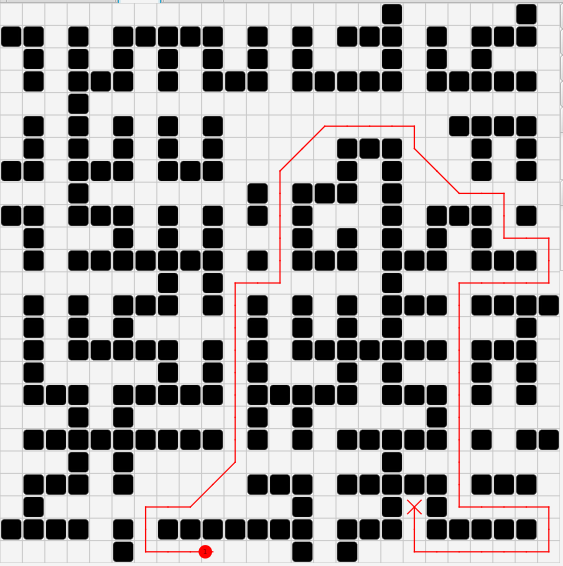
\includegraphics[width=0.7\columnwidth]{img/robopath/astar-simple}
	\caption{Przykładowa ścieżka wyznaczona przez zaimplementowany algorytm A*. Czarne kwadraty reprezentują przeszkody, kolorowe koło - robota, linia łamana - wyznaczoną ścieżkę.}
	\label{fig:robopath-astar-simple}
\end{figure}

% https://en.wikipedia.org/wiki/A*_search_algorithm

% \clearpage{\pagestyle{empty}\cleardoublepage}

% \chapter{Podsumowanie}
\label{ch:podsumowanie}

$TODO$
Większość algorytmów Cooperative Pathfinding opiera się o A*

Algorytmy wprowadzają ograniczenie (błędne założenie), że ruchy trwają tyle samo. Można robić inaczej: podzielić dyskretnie i zaznaczać zajętość pól w wielu kratkach - ale wtedy będzie więcej obliczeń.

Windowed Hierarchical Cooperative A*:
• Cooperative A*
• Hierarchical Heuristic
• Windowed cooperation

The cooperative pathfinding methods are more successful
and find higher quality routes than A* with Local Repair.
Unfortunately, the basic CA* algorithm is costly to compute,

The size of the window has a significant effect on the suc-
cess and performance of the algorithm. With a large win-
dow, WHCA* behaves more like HCA* and the initialisa-
tion time increases. If the window is small, WHCA* be-
haves more like Local Repair A*. The success rate goes
down and the path length increases. The window size pa-
rameter thus provides a spectrum between Local Repair A*
and HCA*. An intermediate choice appears to give the most robust overall performance.
In general, the window size should be set to the duration
of the longest predicted bottleneck. In Real-Time Strategy
games groups of units are often moved together towards a
common destination. In this case the maximum bottleneck
time with cooperative pathfinding (ignoring units in other
groups) is the number of units in the group. If the window
size is lower than this threshold, bottleneck situations may
not be resolved well. If the window size is higher, then some
redundant search will be performed.

Local Repair A* may be an adequate solution for simple en-
vironments with few bottlenecks and few agents. With more
difficult environments, Local Repair A* is inadequate and is
significantly outperformed by Cooperative A* algorithms.

By introducing Hierarchical A* to improve the heuristic and
using windowing to shorten the search, a robust and efficient
algorithm, WHCA*, was developed. WHCA* finds more
successful routes than Local Repair A*, with shorter paths
and fewer cycles.

Although this research was restricted to grid environ-
ments, the algorithms presented here apply equally to more
general pathfinding domains. Any continuous environment
or navigational mesh can be used, so long as each agent’s
route can be planned by discrete motion elements. The grid-
based reservation table is generally applicable, but reserving
mesh intersections may be more appropriate in some cases.
Finally, the cooperative algorithms may be applied in dy-
namic environments, so long as an agent’s route is recom-
puted whenever invalidated by a change to the map.


Cooperative pathfinding is a general technique for coordinating the paths of many units.
It is appropriate whenever there are many units on the same side who are able to
communicate their paths. By planning ahead in time as well as space, units can get out of
each other’s way and avoid any conflicting routes.

Many of the usual enhancements to spatial A* can also be applied to space-time A*.
Moreover, the time dimension gives a whole new set of opportunities for pathfinding
algorithms to explore.

% \clearpage{\pagestyle{empty}\cleardoublepage}

% \phantomsection
% \addcontentsline{toc}{chapter}{Bibliografia}
% \bibliographystyle{unsrt}	
% \bibliography{bibliography}
% \clearpage

% \phantomsection
% \addcontentsline{toc}{chapter}{Wykaz skrótów}
% \chapter*{Wykaz skrótów}

\begin{tabular}{l l}
API & Application Programming Interface \\
SDK & Software Development Kit \\


\end{tabular}

% \clearpage

% \phantomsection
% \addcontentsline{toc}{chapter}{Spis rysunków}
% \listoffigures
% \clearpage

% \phantomsection
% \addcontentsline{toc}{chapter}{Spis tabel}
% \listoftables
% \clearpage